
\documentclass[letterpaper,hide notes,xcolor={table,svgnames},pdftex,10pt]{beamer}
\def\showexamples{t}


%\usepackage[svgnames]{xcolor}

%% Demo talk
%\documentclass[letterpaper,notes=show]{beamer}

\usecolortheme{crane}
\setbeamertemplate{navigation symbols}{}

\usetheme{MyPittsburgh}
%\usetheme{Frankfurt}

%\usepackage{tipa}

\usepackage{hyperref}
\usepackage{graphicx,xspace}
\usepackage[normalem]{ulem}
\usepackage{multicol}
\usepackage{amsmath,amssymb,amsthm,graphicx,xspace}
\newcommand\SF[1]{$\bigstar$\footnote{SF: #1}}

\usepackage[default]{sourcesanspro}
\usepackage[T1]{fontenc}
\usepackage[scaled]{beramono}
\usepackage{tikzpagenodes}

\newcounter{tmpnumSlide}
\newcounter{tmpnumNote}


% old question code
%\newcommand\question[1]{{$\bigstar$ \small \onlySlide{2}{#1}}}
% \newcommand\nquestion[1]{\ifdefined \presentationonly \textcircled{?} \fi \note{\par{\Large \textbf{?}} #1}}
% \newcommand\nanswer[1]{\note{\par{\Large \textbf{A}} #1}}


 \newcommand\mnote[1]{%
   \addtocounter{tmpnumSlide}{1}
   \ifdefined\showcues {~\tiny\fbox{\arabic{tmpnumSlide}}}\fi
   \note{\setlength{\parskip}{1ex}\addtocounter{tmpnumNote}{1}\textbf{\Large \arabic{tmpnumNote}:} {#1\par}}}

\newcommand\mmnote[1]{\note{\setlength{\parskip}{1ex}#1\par}}

%\newcommand\mnote[2][]{\ifdefined\handoutwithnotes {~\tiny\fbox{#1}}\fi
% \note{\setlength{\parskip}{1ex}\textbf{\Large #1:} #2\par}}

%\newcommand\mnote[2][]{{\tiny\fbox{#1}} \note{\setlength{\parskip}{1ex}\textbf{\Large #1:} #2\par}}

\newcommand\mquestion[2]{{~\color{red}\fbox{?}}\note{\setlength{\parskip}{1ex}\par{\Large \textbf{?}} #1} \note{\setlength{\parskip}{1ex}\par{\Large \textbf{A}} #2\par}\ifdefined \presentationonly \pause \fi}

\newcommand\blackboard[1]{%
\ifdefined   \showblackboard
  {#1}
  \else {\begin{center} \fbox{\colorbox{blue!30}{%
         \begin{minipage}{.95\linewidth}%
           \hspace{\stretch{1}} Some space intentionally left blank; done at the blackboard.%
         \end{minipage}}}\end{center}}%
         \fi%
}



%\newcommand\q{\tikz \node[thick,color=black,shape=circle]{?};}
%\newcommand\q{\ifdefined \presentationonly \textcircled{?} \fi}

\usepackage{listings}
\lstset{basicstyle=\footnotesize\ttfamily,
	breaklines=true,
	aboveskip=15pt,
  	belowskip=15pt,
	frame=lines,
	numbers=left, basicstyle=\scriptsize, numberstyle=\tiny, stepnumber=0, numbersep=2pt
}

\usepackage{siunitx}
\newcommand\sius[1]{\num[group-separator = {,}]{#1}\si{\micro\second}}
\newcommand\sims[1]{\num[group-separator = {,}]{#1}\si{\milli\second}}
\newcommand\sins[1]{\num[group-separator = {,}]{#1}\si{\nano\second}}
\sisetup{group-separator = {,}, group-digits = true}

%% -------------------- tikz --------------------
\usepackage{tikz}
\usetikzlibrary{positioning}
\usetikzlibrary{arrows,backgrounds,automata,decorations.shapes,decorations.pathmorphing,decorations.markings,decorations.text,decorations.pathreplacing}

\tikzstyle{place}=[circle,draw=blue!50,fill=blue!20,thick, inner sep=0pt,minimum size=6mm]
\tikzstyle{transition}=[rectangle,draw=black!50,fill=black!20,thick, inner sep=0pt,minimum size=4mm]

\tikzstyle{block}=[rectangle,draw=black, thick, inner sep=5pt]
\tikzstyle{bullet}=[circle,draw=black, fill=black, thin, inner sep=2pt]

\tikzstyle{pre}=[<-,shorten <=1pt,>=stealth',semithick]
\tikzstyle{post}=[->,shorten >=1pt,>=stealth',semithick]
\tikzstyle{bi}=[<->,shorten >=1pt,shorten <=1pt, >=stealth',semithick]

\tikzstyle{mut}=[-,>=stealth',semithick]

\tikzstyle{treereset}=[dashed,->, shorten >=1pt,>=stealth',thin]

\usepackage{ifmtarg}
\usepackage{xifthen}
\makeatletter
% new counter to now which frame it is within the sequence
\newcounter{multiframecounter}
% initialize buffer for previously used frame title
\gdef\lastframetitle{\textit{undefined}}
% new environment for a multi-frame
\newenvironment{multiframe}[1][]{%
\ifthenelse{\isempty{#1}}{%
% if no frame title was set via optional parameter,
% only increase sequence counter by 1
\addtocounter{multiframecounter}{1}%
}{%
% new frame title has been provided, thus
% reset sequence counter to 1 and buffer frame title for later use
\setcounter{multiframecounter}{1}%
\gdef\lastframetitle{#1}%
}%
% start conventional frame environment and
% automatically set frame title followed by sequence counter
\begin{frame}%
\frametitle{\lastframetitle~{\normalfont(\arabic{multiframecounter})}}%
}{%
\end{frame}%
}
\makeatother

\makeatletter
\newdimen\tu@tmpa%
\newdimen\ydiffl%
\newdimen\xdiffl%
\newcommand\ydiff[2]{%
    \coordinate (tmpnamea) at (#1);%
    \coordinate (tmpnameb) at (#2);%
    \pgfextracty{\tu@tmpa}{\pgfpointanchor{tmpnamea}{center}}%
    \pgfextracty{\ydiffl}{\pgfpointanchor{tmpnameb}{center}}%
    \advance\ydiffl by -\tu@tmpa%
}
\newcommand\xdiff[2]{%
    \coordinate (tmpnamea) at (#1);%
    \coordinate (tmpnameb) at (#2);%
    \pgfextractx{\tu@tmpa}{\pgfpointanchor{tmpnamea}{center}}%
    \pgfextractx{\xdiffl}{\pgfpointanchor{tmpnameb}{center}}%
    \advance\xdiffl by -\tu@tmpa%
}
\makeatother
\newcommand{\copyrightbox}[3][r]{%
\begin{tikzpicture}%
\node[inner sep=0pt,minimum size=2em](ciimage){#2};
\usefont{OT1}{phv}{n}{n}\fontsize{4}{4}\selectfont
\ydiff{ciimage.south}{ciimage.north}
\xdiff{ciimage.west}{ciimage.east}
\ifthenelse{\equal{#1}{r}}{%
\node[inner sep=0pt,right=1ex of ciimage.south east,anchor=north west,rotate=90]%
{\raggedleft\color{black!50}\parbox{\the\ydiffl}{\raggedright{}#3}};%
}{%
\ifthenelse{\equal{#1}{l}}{%
\node[inner sep=0pt,right=1ex of ciimage.south west,anchor=south west,rotate=90]%
{\raggedleft\color{black!50}\parbox{\the\ydiffl}{\raggedright{}#3}};%
}{%
\node[inner sep=0pt,below=1ex of ciimage.south west,anchor=north west]%
{\raggedleft\color{black!50}\parbox{\the\xdiffl}{\raggedright{}#3}};%
}
}
\end{tikzpicture}
}


%% --------------------

%\usepackage[excludeor]{everyhook}
%\PushPreHook{par}{\setbox0=\lastbox\llap{MUH}}\box0}

%\vspace*{\stretch{1}

%\setbox0=\lastbox \llap{\textbullet\enskip}\box0}

\setlength{\parskip}{\fill}

\newcommand\noskips{\setlength{\parskip}{1ex}}
\newcommand\doskips{\setlength{\parskip}{\fill}}

\newcommand\xx{\par\vspace*{\stretch{1}}\par}
\newcommand\xxs{\par\vspace*{2ex}\par}
\newcommand\tuple[1]{\langle #1 \rangle}
\newcommand\code[1]{{\sf \footnotesize #1}}
\newcommand\ex[1]{\uline{Example:} \ifdefined \presentationonly \pause \fi
  \ifdefined\showexamples#1\xspace\else{\uline{\hspace*{2cm}}}\fi}

\newcommand\ceil[1]{\lceil #1 \rceil}


\AtBeginSection[]
{
   \begin{frame}
       \frametitle{Outline}
       \tableofcontents[currentsection]
   \end{frame}
}



\pgfdeclarelayer{edgelayer}
\pgfdeclarelayer{nodelayer}
\pgfsetlayers{edgelayer,nodelayer,main}

\tikzstyle{none}=[inner sep=0pt]
\tikzstyle{rn}=[circle,fill=Red,draw=Black,line width=0.8 pt]
\tikzstyle{gn}=[circle,fill=Lime,draw=Black,line width=0.8 pt]
\tikzstyle{yn}=[circle,fill=Yellow,draw=Black,line width=0.8 pt]
\tikzstyle{empty}=[circle,fill=White,draw=Black]
\tikzstyle{bw} = [rectangle, draw, fill=blue!20, 
    text width=4em, text centered, rounded corners, minimum height=2em]
    
    \newcommand{\CcNote}[1]{% longname
	This work is licensed under the \textit{Creative Commons #1 3.0 License}.%
}
\newcommand{\CcImageBy}[1]{%
	\includegraphics[scale=#1]{creative_commons/cc_by_30.pdf}%
}
\newcommand{\CcImageSa}[1]{%
	\includegraphics[scale=#1]{creative_commons/cc_sa_30.pdf}%
}
\newcommand{\CcImageNc}[1]{%
	\includegraphics[scale=#1]{creative_commons/cc_nc_30.pdf}%
}
\newcommand{\CcGroupBySa}[2]{% zoom, gap
	\CcImageBy{#1}\hspace*{#2}\CcImageNc{#1}\hspace*{#2}\CcImageSa{#1}%
}
\newcommand{\CcLongnameByNcSa}{Attribution-NonCommercial-ShareAlike}

\newenvironment{changemargin}[1]{% 
  \begin{list}{}{% 
    \setlength{\topsep}{0pt}% 
    \setlength{\leftmargin}{#1}% 
    \setlength{\rightmargin}{1em}
    \setlength{\listparindent}{\parindent}% 
    \setlength{\itemindent}{\parindent}% 
    \setlength{\parsep}{\parskip}% 
  }% 
  \item[]}{\end{list}} 




% Custom packages
\usepackage{xcolor}
\definecolor{solarizedBase03}{HTML}{FFFFFF}
\definecolor{solarizedBase02}{HTML}{000000}
\definecolor{solarizedBase00}{HTML}{657B83}
\definecolor{solarizedBase0}{HTML}{000000}
\definecolor{solarizedBase1}{HTML}{93A1A1}
\definecolor{solarizedBase3}{HTML}{FDF6E3}


\usepackage[listings]{tcolorbox}
\newtcbinputlisting{\codelisting}[2][]{
    listing file={#2},
    colback=solarizedBase03,
    colframe=solarizedBase02,
    colupper=solarizedBase0,
    fonttitle=\bfseries\color{solarizedBase1},
    listing options={basicstyle=\ttfamily\footnotesize},
    listing only,
    #1
}

\title{Lecture 22 --- GPU Programming / OpenCL }

\author{Patrick Lam \\ \small \texttt{patrick.lam@uwaterloo.ca}}
\institute{Department of Electrical and Computer Engineering \\
  University of Waterloo}
\date{\today}


\begin{document}

\begin{frame}
  \titlepage

 \end{frame}


%%%%%%%%%%%%%%%%%%%%%%%%%%%%%%%%%%%%%%%%%%%%%%%%%%%%%%%%%%%%%%%%%%%%%%%%%%%%%%%%
\part{OpenCL concepts}
\frame{\partpage}
%%%%%%%%%%%%%%%%%%%%%%%%%%%%%%%%%%%%%%%%%%%%%%%%%%%%%%%%%%%%%%%%%%%%%%%%%%%%%%%%

%%%%%%%%%%%%%%%%%%%%%%%%%%%%%%%%%%%%%%%%%%%%%%%%%%%%%%%%%%%%%%%%%%%%%%%%%%%%%%%%
\begin{frame}
  \frametitle{Introduction}


     \structure{OpenCL}: coding on a heterogeneous architecture.
      \begin{itemize}
        \item No longer just programming the CPU;\\ will also leverage the GPU.
      \end{itemize}
      OpenCL = Open Computing Language.\\
      Usable on both NVIDIA and AMD GPUs.
      
    \begin{center}
	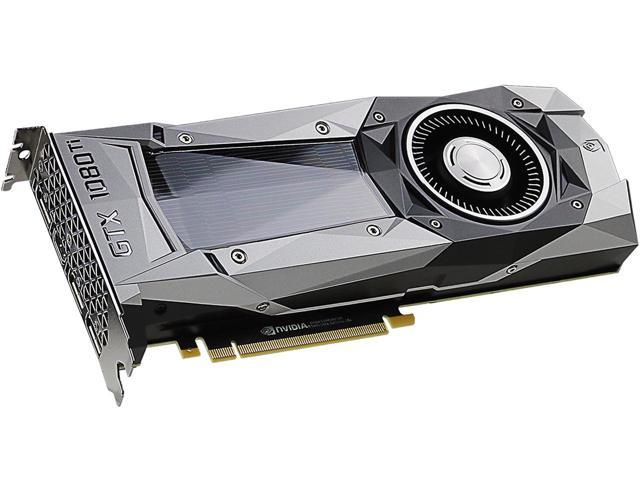
\includegraphics[width=0.5\textwidth]{images/gpu.jpg}
	\end{center}

\end{frame}
%%%%%%%%%%%%%%%%%%%%%%%%%%%%%%%%%%%%%%%%%%%%%%%%%%%%%%%%%%%%%%%%%%%%%%%%%%%%%%%%

%%%%%%%%%%%%%%%%%%%%%%%%%%%%%%%%%%%%%%%%%%%%%%%%%%%%%%%%%%%%%%%%%%%%%%%%%%%%%%%%
\begin{frame}
  \frametitle{SIMT}



  Another term you may see vendors using:

  \begin{itemize}
    \item {\bf S}ingle {\bf I}nstruction, {\bf M}ultiple {\bf T}hreads.
    \item Runs on a vector of data.
    \item Similar to SIMD instructions (e.g. SSE).\\
     However, the vector is spread out over the GPU.
  \end{itemize}

\end{frame}
%%%%%%%%%%%%%%%%%%%%%%%%%%%%%%%%%%%%%%%%%%%%%%%%%%%%%%%%%%%%%%%%%%%%%%%%%%%%%%%%

%%%%%%%%%%%%%%%%%%%%%%%%%%%%%%%%%%%%%%%%%%%%%%%%%%%%%%%%%%%%%%%%%%%%%%%%%%%%%%%%
\begin{frame}
  \frametitle{Other Heterogeneous Programming Examples}


\begin{itemize}
\item PlayStation 3 Cell\\
\item CUDA
\end{itemize}
~\\[1em]
[PS4: back to a regular CPU/GPU system, albeit on one chip.]

See \url{https://www.youtube.com/watch?v=zW3XawAsaeU} for details on why it was hard to program for the PS3!

\end{frame}
%%%%%%%%%%%%%%%%%%%%%%%%%%%%%%%%%%%%%%%%%%%%%%%%%%%%%%%%%%%%%%%%%%%%%%%%%%%%%%%%

%%%%%%%%%%%%%%%%%%%%%%%%%%%%%%%%%%%%%%%%%%%%%%%%%%%%%%%%%%%%%%%%%%%%%%%%%%%%%%%%
\begin{frame}
  \frametitle{(PS3) Cell Overview}


  Cell consists of:
  \begin{itemize}
    \item a PowerPC core; and
    \item 8 SIMD co-processors.
  \end{itemize}


  \begin{center}
    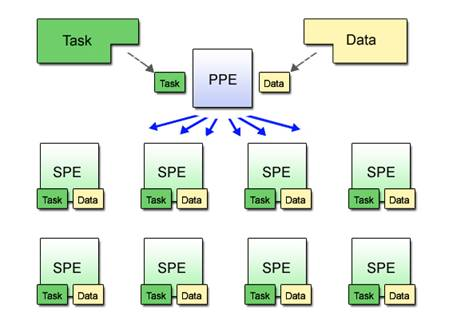
\includegraphics[scale=0.5]{images/cell}
  \end{center}
  \hfill (from the Linux Cell documentation)

\end{frame}
%%%%%%%%%%%%%%%%%%%%%%%%%%%%%%%%%%%%%%%%%%%%%%%%%%%%%%%%%%%%%%%%%%%%%%%%%%%%%%%%

%%%%%%%%%%%%%%%%%%%%%%%%%%%%%%%%%%%%%%%%%%%%%%%%%%%%%%%%%%%%%%%%%%%%%%%%%%%%%%%%
\begin{frame}
  \frametitle{CUDA Overview}
  

     Compute Unified Device Architecture:\\
     NVIDIA's architecture for processing on GPUs.\\[1em]

     ``C for CUDA'' predates OpenCL,\\
     NVIDIA supports it first and foremost.
      \begin{itemize}
        \item May be faster than OpenCL on NVIDIA hardware.
        \item API allows you to use (most) C++ features in CUDA; \\
          OpenCL has more restrictions.
      \end{itemize}

\end{frame}
%%%%%%%%%%%%%%%%%%%%%%%%%%%%%%%%%%%%%%%%%%%%%%%%%%%%%%%%%%%%%%%%%%%%%%%%%%%%%%%%

%%%%%%%%%%%%%%%%%%%%%%%%%%%%%%%%%%%%%%%%%%%%%%%%%%%%%%%%%%%%%%%%%%%%%%%%%%%%%%%%
\begin{frame}
  \frametitle{GPU Programming Model}



  The abstract model is simple:

  \begin{itemize}
    \item Write the code for the parallel computation ({\it kernel}) \\
      \qquad separately from main code.
    \item Transfer the data to the GPU co-processor \\
      \qquad (or execute it on the CPU).
    \item Wait \ldots
    \item Transfer the results back.
  \end{itemize}

\end{frame}
%%%%%%%%%%%%%%%%%%%%%%%%%%%%%%%%%%%%%%%%%%%%%%%%%%%%%%%%%%%%%%%%%%%%%%%%%%%%%%%%

%%%%%%%%%%%%%%%%%%%%%%%%%%%%%%%%%%%%%%%%%%%%%%%%%%%%%%%%%%%%%%%%%%%%%%%%%%%%%%%%
\begin{frame}
  \frametitle{Data Parallelism}


  \begin{itemize}
    \item Key idea: evaluate a function (or {\it kernel}) \\
     \qquad over a set of points (data).\\

\begin{center}

\begin{tikzpicture}
\foreach \x in {0,0.25,...,2}
  \foreach \y in {0,0.25,...,2}
    \draw (\x, \y) circle (0.25mm);
\end{tikzpicture}
\end{center}

      Another example of data parallelism.\\[1em]
    \item Another name for the set of points: {\it index space}.
    \item Each point corresponds to a {\bf work-item}.
  \end{itemize}~\\[1em]

  Note: OpenCL also supports {\it task parallelism} (using different kernels),
  but documentation is sparse.

\end{frame}
%%%%%%%%%%%%%%%%%%%%%%%%%%%%%%%%%%%%%%%%%%%%%%%%%%%%%%%%%%%%%%%%%%%%%%%%%%%%%%%%

%%%%%%%%%%%%%%%%%%%%%%%%%%%%%%%%%%%%%%%%%%%%%%%%%%%%%%%%%%%%%%%%%%%%%%%%%%%%%%%%
\begin{frame}
  \frametitle{Work-Items}


    \structure{Work-item}: the fundamental unit of work in OpenCL.\\
    Stored in an {\it n}-dimensional grid (ND-Range); 2D on previous slide.\\[1em]

    OpenCL spawns a bunch of threads to handle work-items.
    
    \begin{center}
	
\includegraphics[width=0.2\textwidth]{images/peon.jpeg}\\
	\hfill ``Ready to work!''
	\end{center}
    
\end{frame}
    
\begin{frame}
\frametitle{Work-Items}
    
    When executing, the range is divided into {\bf work-groups}, which
      execute on the same compute unit.\\[1em]

    The set of compute units (or cores) is called something different
          depending on the manufacturer.
          \begin{itemize}
            \item NVIDIA - {\it warp}
            \item AMD/ATI - {\it wavefront}
          \end{itemize}

\end{frame}
%%%%%%%%%%%%%%%%%%%%%%%%%%%%%%%%%%%%%%%%%%%%%%%%%%%%%%%%%%%%%%%%%%%%%%%%%%%%%%%%

%%%%%%%%%%%%%%%%%%%%%%%%%%%%%%%%%%%%%%%%%%%%%%%%%%%%%%%%%%%%%%%%%%%%%%%%%%%%%%%%
\begin{frame}
  \frametitle{Work-Items: Three more details}


  One thread per work item, each with a different thread ID.\\[1em]

  You can say how to divide the ND-Range into work-groups, \\
  or the system can do it for you.\\[1em]

  Scheduler assigns work-items to warps/wavefronts until no more left.


\end{frame}
%%%%%%%%%%%%%%%%%%%%%%%%%%%%%%%%%%%%%%%%%%%%%%%%%%%%%%%%%%%%%%%%%%%%%%%%%%%%%%%%

%%%%%%%%%%%%%%%%%%%%%%%%%%%%%%%%%%%%%%%%%%%%%%%%%%%%%%%%%%%%%%%%%%%%%%%%%%%%%%%%
\begin{frame}
  \frametitle{Shared Memory}


  There are many different types of memory available to you:


\begin{itemize}
\item private memory
\item local memory
\item global memory
\item constant memory
\end{itemize}

There is also host memory (normal memory);\\ usually contains app data.

\end{frame}
%%%%%%%%%%%%%%%%%%%%%%%%%%%%%%%%%%%%%%%%%%%%%%%%%%%%%%%%%%%%%%%%%%%%%%%%%%%%%%%%

%%%%%%%%%%%%%%%%%%%%%%%%%%%%%%%%%%%%%%%%%%%%%%%%%%%%%%%%%%%%%%%%%%%%%%%%%%%%%%%%
\begin{frame}[fragile]
  \frametitle{Example Kernel}


    Here's some traditional code to evaluate $C_i = A_iB_i$:

\begin{lstlisting}[language=C]
  void traditional_mul(int n, 
                       const float *a, 
                       const float *b, 
                       float *c) {
    int i;
    for (i = 0; i < n; i++) c[i] = a[i] * b[i];
  }
\end{lstlisting}


And as a kernel:
\begin{lstlisting}[language=C]
  kernel void opencl_mul(global const float *a, 
                         global const float *b,
                         global float *c) {
    int id = get_global_id(0);  // dimension 0
    c[id] = a[id] * b[id];
  }
\end{lstlisting}


\end{frame}
%%%%%%%%%%%%%%%%%%%%%%%%%%%%%%%%%%%%%%%%%%%%%%%%%%%%%%%%%%%%%%%%%%%%%%%%%%%%%%%%

%%%%%%%%%%%%%%%%%%%%%%%%%%%%%%%%%%%%%%%%%%%%%%%%%%%%%%%%%%%%%%%%%%%%%%%%%%%%%%%%
\begin{frame}
  \frametitle{Restrictions when writing kernels in OpenCL}


  It's mostly C, but:
  \begin{itemize}
    \item No function pointers.
    \item No bit-fields.
    \item No variable-length arrays.
    \item No recursion.
    \item No standard headers.
  \end{itemize}

\end{frame}
%%%%%%%%%%%%%%%%%%%%%%%%%%%%%%%%%%%%%%%%%%%%%%%%%%%%%%%%%%%%%%%%%%%%%%%%%%%%%%%%

%%%%%%%%%%%%%%%%%%%%%%%%%%%%%%%%%%%%%%%%%%%%%%%%%%%%%%%%%%%%%%%%%%%%%%%%%%%%%%%%
\begin{frame}
  \frametitle{OpenCL's Additions to C in Kernels}


In kernels, you can also use:
  \begin{itemize}
    \item Work-items.
    \item Work-groups.
    \item Vectors.
    \item Synchronization.
    \item Declarations of memory type.
    \item Kernel-specific library.
  \end{itemize}

\end{frame}
%%%%%%%%%%%%%%%%%%%%%%%%%%%%%%%%%%%%%%%%%%%%%%%%%%%%%%%%%%%%%%%%%%%%%%%%%%%%%%%%


\begin{frame}
\frametitle{Branches}

The hardware will execute \emph{all} branches that any thread in a warp
      executes---can be slow!\\[1em]


\begin{center}
	
\includegraphics[width=0.5\textwidth]{images/whynotboth.jpg}
\end{center}

\end{frame}


%%%%%%%%%%%%%%%%%%%%%%%%%%%%%%%%%%%%%%%%%%%%%%%%%%%%%%%%%%%%%%%%%%%%%%%%%%%%%%%%
\begin{frame}
  \frametitle{Branches in kernels}

  \codelisting{images/branch.cpp}

    
    In other words: an {\tt if} statement will cause each thread to execute
      both branches; we keep only the result of the taken branch.\\[1em]


\end{frame}
%%%%%%%%%%%%%%%%%%%%%%%%%%%%%%%%%%%%%%%%%%%%%%%%%%%%%%%%%%%%%%%%%%%%%%%%%%%%%%%%

%%%%%%%%%%%%%%%%%%%%%%%%%%%%%%%%%%%%%%%%%%%%%%%%%%%%%%%%%%%%%%%%%%%%%%%%%%%%%%%%
\begin{frame}
  \frametitle{Loops in kernels}

  \codelisting{images/loop.cpp}

      
    A loop will cause the workgroup to wait for the maximum number of
      iterations of the loop in any work-item.\\[1em]

  Note: when you set up work-groups, best to arrange for all work-items in
  a workgroup to execute the same branches \& loops.

\end{frame}
%%%%%%%%%%%%%%%%%%%%%%%%%%%%%%%%%%%%%%%%%%%%%%%%%%%%%%%%%%%%%%%%%%%%%%%%%%%%%%%%

%%%%%%%%%%%%%%%%%%%%%%%%%%%%%%%%%%%%%%%%%%%%%%%%%%%%%%%%%%%%%%%%%%%%%%%%%%%%%%%%
\begin{frame}
  \frametitle{Synchronization}



Different workgroups execute independently.\\
You can only put barriers and memory fences between work-items in the
      same workgroup.\\[1em]

OpenCL supports:
  \begin{itemize}
    \item Memory fences (load and store).
    \item Barriers.
    \item {\tt volatile} (beware!)
  \end{itemize}

\end{frame}
%%%%%%%%%%%%%%%%%%%%%%%%%%%%%%%%%%%%%%%%%%%%%%%%%%%%%%%%%%%%%%%%%%%%%%%%%%%%%%%%

%%%%%%%%%%%%%%%%%%%%%%%%%%%%%%%%%%%%%%%%%%%%%%%%%%%%%%%%%%%%%%%%%%%%%%%%%%%%%%%%
\part{Programming with OpenCL}
\frame{\partpage}
%%%%%%%%%%%%%%%%%%%%%%%%%%%%%%%%%%%%%%%%%%%%%%%%%%%%%%%%%%%%%%%%%%%%%%%%%%%%%%%%


%%%%%%%%%%%%%%%%%%%%%%%%%%%%%%%%%%%%%%%%%%%%%%%%%%%%%%%%%%%%%%%%%%%%%%%%%%%%%%%%
\begin{frame}
  \frametitle{Introduction}



  Today, we'll see how to program with OpenCL.

  \begin{itemize}
    \item We're using OpenCL 1.1.
    \item There is a lot of initialization and querying.
    \item When you compile your program, include {\tt -lOpenCL}.
  \end{itemize}~\\[1em]

  You can find the official documentation here:

  \qquad \url{http://www.khronos.org/opencl/}

  More specifically:\\
  \quad {\scriptsize \url{http://www.khronos.org/registry/cl/sdk/1.1/docs/man/xhtml/}}
  \vfill
  Let's just dive into an example.

\end{frame}
%%%%%%%%%%%%%%%%%%%%%%%%%%%%%%%%%%%%%%%%%%%%%%%%%%%%%%%%%%%%%%%%%%%%%%%%%%%%%%%%

%%%%%%%%%%%%%%%%%%%%%%%%%%%%%%%%%%%%%%%%%%%%%%%%%%%%%%%%%%%%%%%%%%%%%%%%%%%%%%%%
\begin{frame}
  \frametitle{First, reminders}


  \begin{itemize}
    \item All data belongs to an {\bf NDRange}.
    \item The range can be divided into {\bf work-groups}. (in software)
    \item The work-groups run on {\bf wavefronts/warps}. (in hardware)
    \item Each wavefront/warp executes {\bf work-items}.
  \end{itemize}~\\[1em]

  \alert{All} branches in a wavefront/warp should execute the same path.~\\[1em]

  If an iteration of a loop takes {\tt t}:\\ when one work-item executes 100
    iterations,\\ the total time to complete the wavefront/warp is {\tt 100t.}

\end{frame}
%%%%%%%%%%%%%%%%%%%%%%%%%%%%%%%%%%%%%%%%%%%%%%%%%%%%%%%%%%%%%%%%%%%%%%%%%%%%%%%%

\part{Simple Example}
\frame{\partpage}
%%%%%%%%%%%%%%%%%%%%%%%%%%%%%%%%%%%%%%%%%%%%%%%%%%%%%%%%%%%%%%%%%%%%%%%%%%%%%%%%
\begin{frame}[fragile]
  \frametitle{Simple Example (1)}


\begin{lstlisting}[language=C]
// Note by PL: don't use this example as a template;
// it uses the C bindings! Instead, use the C++ bindings.
// source: pages 1-9 through 1-11,
// http://developer.amd.com/wordpress/media/2013/07/
//     AMD_Accelerated_Parallel_Processing_OpenCL_
//     Programming_Guide-rev-2.7.pdf

#include <CL/cl.h>
#include <stdio.h>

#define NWITEMS 512

// A simple memset kernel
const char *source =
"__kernel void memset( __global uint *dst )             \n"
"{                                                      \n"
"   dst[get_global_id(0)] = get_global_id(0);           \n"
"}                                                      \n";

int main(int argc, char ** argv)
{
   // 1. Get a platform.
   cl_platform_id platform;
   clGetPlatformIDs(1, &platform, NULL);
  \end{lstlisting}

\end{frame}
%%%%%%%%%%%%%%%%%%%%%%%%%%%%%%%%%%%%%%%%%%%%%%%%%%%%%%%%%%%%%%%%%%%%%%%%%%%%%%%%

%%%%%%%%%%%%%%%%%%%%%%%%%%%%%%%%%%%%%%%%%%%%%%%%%%%%%%%%%%%%%%%%%%%%%%%%%%%%%%%%
\begin{frame}
  \frametitle{Explanation (1)}


    Include the OpenCL header.\\[1em]

    Request a platform (also known as a host).\\[1em]

    A platform contains {\it compute devices}:
      \begin{itemize}
        \item GPUs or CPUs.
      \end{itemize}

\end{frame}
%%%%%%%%%%%%%%%%%%%%%%%%%%%%%%%%%%%%%%%%%%%%%%%%%%%%%%%%%%%%%%%%%%%%%%%%%%%%%%%%

%%%%%%%%%%%%%%%%%%%%%%%%%%%%%%%%%%%%%%%%%%%%%%%%%%%%%%%%%%%%%%%%%%%%%%%%%%%%%%%%
\begin{frame}[fragile]
  \frametitle{Simple Example (2)}



  \begin{lstlisting}[language=C]
   // 2. Find a gpu device.
   cl_device_id device;
   clGetDeviceIDs(platform, CL_DEVICE_TYPE_GPU,
                  1,
                  &device,
                  NULL);

   // 3. Create a context and command queue on that device.
   cl_context context = clCreateContext(NULL,
                                        1,
                                        &device,
                                        NULL, NULL, NULL);
   cl_command_queue queue = clCreateCommandQueue(context,
                                                 device,
                                                 0, NULL);
  \end{lstlisting}

\end{frame}
%%%%%%%%%%%%%%%%%%%%%%%%%%%%%%%%%%%%%%%%%%%%%%%%%%%%%%%%%%%%%%%%%%%%%%%%%%%%%%%%

%%%%%%%%%%%%%%%%%%%%%%%%%%%%%%%%%%%%%%%%%%%%%%%%%%%%%%%%%%%%%%%%%%%%%%%%%%%%%%%%
\begin{frame}
  \frametitle{Explanation (2)}


    Request a GPU device.\\[1em]

    Request a OpenCL context (representing all of OpenCL's state).\\[1em]

    Create a command-queue: \\
 get OpenCL to do work by telling it to run
      a kernel in a queue.

\end{frame}
%%%%%%%%%%%%%%%%%%%%%%%%%%%%%%%%%%%%%%%%%%%%%%%%%%%%%%%%%%%%%%%%%%%%%%%%%%%%%%%%

%%%%%%%%%%%%%%%%%%%%%%%%%%%%%%%%%%%%%%%%%%%%%%%%%%%%%%%%%%%%%%%%%%%%%%%%%%%%%%%%
\begin{frame}[fragile]
  \frametitle{Simple Example (3)}


  \begin{lstlisting}[language=C]
   // 4. Perform runtime source compilation, and obtain
   //    kernel entry point.
   cl_program program = clCreateProgramWithSource(context,
                                                  1,
                                                  &source,
                                                  NULL,
                                                  NULL);
   clBuildProgram(program, 1, &device, NULL, NULL, NULL);
   cl_kernel kernel = clCreateKernel(program, "memset",
                                     NULL);

   // 5. Create a data buffer.
   cl_mem buffer = clCreateBuffer(context,
                                  CL_MEM_WRITE_ONLY,
                                  NWITEMS * sizeof(cl_uint),
                                  NULL, NULL);
  \end{lstlisting}

\end{frame}
%%%%%%%%%%%%%%%%%%%%%%%%%%%%%%%%%%%%%%%%%%%%%%%%%%%%%%%%%%%%%%%%%%%%%%%%%%%%%%%%

%%%%%%%%%%%%%%%%%%%%%%%%%%%%%%%%%%%%%%%%%%%%%%%%%%%%%%%%%%%%%%%%%%%%%%%%%%%%%%%%
\begin{frame}
  \frametitle{Explanation (3)}


    We create an OpenCL ``program'' (runs on the compute unit):
      \begin{itemize}
        \item kernels;
        \item functions; and
        \item declarations.
      \end{itemize}
    In this case, we create a kernel called {\tt memset} from {\tt source}.\\
    OpenCL may also create programs from binaries\\
      (may~be~in~intermediate~representation).\\[1em]

    Next, we need a {\it data buffer} (enables inter-device communication).\\[1em]

    This program does not have any input, \\
      so we don't put anything into
      the buffer (just declare its size).

\end{frame}
%%%%%%%%%%%%%%%%%%%%%%%%%%%%%%%%%%%%%%%%%%%%%%%%%%%%%%%%%%%%%%%%%%%%%%%%%%%%%%%%

%%%%%%%%%%%%%%%%%%%%%%%%%%%%%%%%%%%%%%%%%%%%%%%%%%%%%%%%%%%%%%%%%%%%%%%%%%%%%%%%
\begin{frame}[fragile]
  \frametitle{Simple Example (4)}



  \begin{lstlisting}[language=C]
   // 6. Launch the kernel. Let OpenCL pick the local work
   //    size.
   size_t global_work_size = NWITEMS;
   clSetKernelArg(kernel,0, sizeof(buffer), (void*)&buffer);
   clEnqueueNDRangeKernel(queue,
                          kernel,
                          1,    // dimensions
                          NULL, // initial offsets
                          &global_work_size, // number of
                                             // work-items
                          NULL, // work-items per work-group
                          0, NULL, NULL);  // events
   clFinish(queue);

   // 7. Look at the results via synchronous buffer map.
   cl_uint *ptr;
   ptr = (cl_uint *)clEnqueueMapBuffer(queue, buffer,
                                       CL_TRUE, CL_MAP_READ,
                                       0, NWITEMS *
                                       sizeof(cl_uint),
                                       0, NULL, NULL, NULL);
  \end{lstlisting}

\end{frame}
%%%%%%%%%%%%%%%%%%%%%%%%%%%%%%%%%%%%%%%%%%%%%%%%%%%%%%%%%%%%%%%%%%%%%%%%%%%%%%%%

%%%%%%%%%%%%%%%%%%%%%%%%%%%%%%%%%%%%%%%%%%%%%%%%%%%%%%%%%%%%%%%%%%%%%%%%%%%%%%%%
\begin{frame}
  \frametitle{Explanation (4)}


    Set kernel arguments to {\tt buffer}.\\[.5em]
    We launch the kernel, enqueuing the 1-dimensional index~space starting
      at 0.\\[.5em]
    We specify that the index space has {\tt NWITEMS} elements; \\and not to
      subdivide the program into work-groups.\\[.5em]
    There is also an event interface, which we do not use.\\[2em]

    We copy the results back; call is blocking ({\tt CL\_TRUE});\\
    \qquad hence we don't need an explicit {\tt clFinish()} call.\\[.5em]
    We specify that we want to read the results back into buffer.

\end{frame}
%%%%%%%%%%%%%%%%%%%%%%%%%%%%%%%%%%%%%%%%%%%%%%%%%%%%%%%%%%%%%%%%%%%%%%%%%%%%%%%%

%%%%%%%%%%%%%%%%%%%%%%%%%%%%%%%%%%%%%%%%%%%%%%%%%%%%%%%%%%%%%%%%%%%%%%%%%%%%%%%%
\begin{frame}[fragile]
  \frametitle{Simple Example (5)}



  \begin{lstlisting}[language=C]
   int i;
   for(i=0; i < NWITEMS; i++)
       printf("%d %d\n", i, ptr[i]);
   return 0;
}
  \end{lstlisting}

  \begin{itemize}
    \item The program simply prints {\tt 0 0}, {\tt 1 1}, \ldots, {\tt 511 511}.
    \item Note: I didn't clean up or include error handling\\ for any of the
      OpenCL functions.
  \end{itemize}

\end{frame}
%%%%%%%%%%%%%%%%%%%%%%%%%%%%%%%%%%%%%%%%%%%%%%%%%%%%%%%%%%%%%%%%%%%%%%%%%%%%%%%%

\part{Another Example}
\frame{\partpage}

%%%%%%%%%%%%%%%%%%%%%%%%%%%%%%%%%%%%%%%%%%%%%%%%%%%%%%%%%%%%%%%%%%%%%%%%%%%%%%%%
\begin{frame}
  \frametitle{C++ Bindings}


    If we use the C++ bindings, we'll get automatic \\ resource release and
      exceptions.
      \begin{itemize}
        \item C++ likes to use the RAII style
          (resource~allocation~is~initialization).
      \end{itemize}~\\
    Change the header to {\tt CL/cl.hpp} and define
      {\tt \_\_CL\_ENABLE\_EXCEPTIONS}.\\[.5em]
    We'd also like to store our kernel in a file instead of a string.\\[.5em]
    The C API is not so nice to work with.

\end{frame}
%%%%%%%%%%%%%%%%%%%%%%%%%%%%%%%%%%%%%%%%%%%%%%%%%%%%%%%%%%%%%%%%%%%%%%%%%%%%%%%%

%%%%%%%%%%%%%%%%%%%%%%%%%%%%%%%%%%%%%%%%%%%%%%%%%%%%%%%%%%%%%%%%%%%%%%%%%%%%%%%%
\begin{frame}[fragile]
  \frametitle{Vector Addition Kernel}


    Let's write a kernel that adds two vectors and stores the result.\\
    This kernel will go in the file {\tt vector\_add\_kernel.cl}.

  \begin{lstlisting}[language=C]
__kernel void vector_add(__global const int *A,
                         __global const int *B,
                         __global int *C) {
 
    // Get the index of the current element to be processed
    int i = get_global_id(0);
 
    // Do the operation
    C[i] = A[i] + B[i];
}
  \end{lstlisting}

    Other possible qualifiers: {\tt local}, {\tt constant} and {\tt private}.


\end{frame}
%%%%%%%%%%%%%%%%%%%%%%%%%%%%%%%%%%%%%%%%%%%%%%%%%%%%%%%%%%%%%%%%%%%%%%%%%%%%%%%%

%%%%%%%%%%%%%%%%%%%%%%%%%%%%%%%%%%%%%%%%%%%%%%%%%%%%%%%%%%%%%%%%%%%%%%%%%%%%%%%%
\begin{frame}[fragile]
  \frametitle{Vector Addition (1)}


  \begin{lstlisting}[language=C++]
// Vector add example, C++ bindings (use these!)
// source:
//  http://www.thebigblob.com/getting-started-
//        with-opencl-and-gpu-computing/

#define __CL_ENABLE_EXCEPTIONS

#include <CL/cl.hpp>

#include <iostream>
#include <fstream>
#include <string>
#include <utility>
#include <vector>
 
int main() {
    // Create the two input vectors
    const int LIST_SIZE = 1000;
    int *A = new int[LIST_SIZE]; 
    int *B = new int[LIST_SIZE];
    for(int i = 0; i < LIST_SIZE; i++) {
        A[i] = i;
        B[i] = LIST_SIZE - i;
    }
  \end{lstlisting}

\end{frame}
%%%%%%%%%%%%%%%%%%%%%%%%%%%%%%%%%%%%%%%%%%%%%%%%%%%%%%%%%%%%%%%%%%%%%%%%%%%%%%%%

%%%%%%%%%%%%%%%%%%%%%%%%%%%%%%%%%%%%%%%%%%%%%%%%%%%%%%%%%%%%%%%%%%%%%%%%%%%%%%%%
\begin{frame}[fragile]
  \frametitle{Vector Addition (2)}


  \begin{lstlisting}[language=C++]
    try { 
        // Get available platforms
        std::vector<cl::Platform> platforms;
        cl::Platform::get(&platforms);

        // Select the default platform and create a context
        // using this platform and the GPU
        cl_context_properties cps[3] = { 
            CL_CONTEXT_PLATFORM, 
            (cl_context_properties)(platforms[0])(), 
            0 
        };
        cl::Context context(CL_DEVICE_TYPE_GPU, cps);
 
        // Get a list of devices on this platform
        std::vector<cl::Device> devices =
            context.getInfo<CL_CONTEXT_DEVICES>();
 
        // Create a command queue and use the first device
        cl::CommandQueue queue = cl::CommandQueue(context,
            devices[0]);
  \end{lstlisting}

\end{frame}
%%%%%%%%%%%%%%%%%%%%%%%%%%%%%%%%%%%%%%%%%%%%%%%%%%%%%%%%%%%%%%%%%%%%%%%%%%%%%%%%

%%%%%%%%%%%%%%%%%%%%%%%%%%%%%%%%%%%%%%%%%%%%%%%%%%%%%%%%%%%%%%%%%%%%%%%%%%%%%%%%
\begin{frame}
  \frametitle{Explanation (2)}



    You can define {\tt \_\_NO\_STD\_VECTOR} and use {\tt cl::vector}
      (same with strings).\\[1em]
    You can enable profiling by adding {\tt CL\_QUEUE\_PROFILING\_ENABLE}
      as 3rd argument to {\tt queue}.

\end{frame}
%%%%%%%%%%%%%%%%%%%%%%%%%%%%%%%%%%%%%%%%%%%%%%%%%%%%%%%%%%%%%%%%%%%%%%%%%%%%%%%%

%%%%%%%%%%%%%%%%%%%%%%%%%%%%%%%%%%%%%%%%%%%%%%%%%%%%%%%%%%%%%%%%%%%%%%%%%%%%%%%%
\begin{frame}[fragile]
  \frametitle{Vector Addition (3)}



  \begin{lstlisting}[language=C++]
        // Read source file
        std::ifstream sourceFile("vector_add_kernel.cl");
        std::string sourceCode(
            std::istreambuf_iterator<char>(sourceFile),
            (std::istreambuf_iterator<char>())
        );
        cl::Program::Sources source(
            1,
            std::make_pair(sourceCode.c_str(),
                           sourceCode.length()+1)
        );
 
        // Make program of the source code in the context
        cl::Program program = cl::Program(context, source);
 
        // Build program for these specific devices
        program.build(devices);
 
        // Make kernel
        cl::Kernel kernel(program, "vector_add");
  \end{lstlisting}

\end{frame}
%%%%%%%%%%%%%%%%%%%%%%%%%%%%%%%%%%%%%%%%%%%%%%%%%%%%%%%%%%%%%%%%%%%%%%%%%%%%%%%%

%%%%%%%%%%%%%%%%%%%%%%%%%%%%%%%%%%%%%%%%%%%%%%%%%%%%%%%%%%%%%%%%%%%%%%%%%%%%%%%%
\begin{frame}[fragile]
  \frametitle{Vector Addition (4)}


  \begin{lstlisting}[language=C++]
        // Create memory buffers
        cl::Buffer bufferA = cl::Buffer(
            context,
            CL_MEM_READ_ONLY,
            LIST_SIZE * sizeof(int)
        );
        cl::Buffer bufferB = cl::Buffer(
            context,
            CL_MEM_READ_ONLY,
            LIST_SIZE * sizeof(int)
        );
        cl::Buffer bufferC = cl::Buffer(
            context,
            CL_MEM_WRITE_ONLY,
            LIST_SIZE * sizeof(int)
        );
  \end{lstlisting}


\end{frame}
%%%%%%%%%%%%%%%%%%%%%%%%%%%%%%%%%%%%%%%%%%%%%%%%%%%%%%%%%%%%%%%%%%%%%%%%%%%%%%%%

%%%%%%%%%%%%%%%%%%%%%%%%%%%%%%%%%%%%%%%%%%%%%%%%%%%%%%%%%%%%%%%%%%%%%%%%%%%%%%%%
\begin{frame}[fragile]
  \frametitle{Vector Addition (5)}

  \begin{lstlisting}[language=C++]
        // Copy lists A and B to the memory buffers
        queue.enqueueWriteBuffer(
            bufferA,
            CL_TRUE,
            0,
            LIST_SIZE * sizeof(int),
            A
        );
        queue.enqueueWriteBuffer(
            bufferB,
            CL_TRUE,
            0,
            LIST_SIZE * sizeof(int),
            B
        );
 
        // Set arguments to kernel
        kernel.setArg(0, bufferA);
        kernel.setArg(1, bufferB);
        kernel.setArg(2, bufferC);
  \end{lstlisting}

\end{frame}
%%%%%%%%%%%%%%%%%%%%%%%%%%%%%%%%%%%%%%%%%%%%%%%%%%%%%%%%%%%%%%%%%%%%%%%%%%%%%%%%

%%%%%%%%%%%%%%%%%%%%%%%%%%%%%%%%%%%%%%%%%%%%%%%%%%%%%%%%%%%%%%%%%%%%%%%%%%%%%%%%
\begin{frame}
  \frametitle{Explanation (5)}


  {\tt enqueue*Buffer} arguments:

  \begin{itemize}
    \item {\it buffer}
    \item {\tt cl\_ bool} {\it blocking\_write}
    \item {\tt ::size\_t} {\it offset}
    \item {\tt ::size\_t} {\it size}
    \item {\tt const void *} {\it ptr}
  \end{itemize}

\end{frame}
%%%%%%%%%%%%%%%%%%%%%%%%%%%%%%%%%%%%%%%%%%%%%%%%%%%%%%%%%%%%%%%%%%%%%%%%%%%%%%%%

%%%%%%%%%%%%%%%%%%%%%%%%%%%%%%%%%%%%%%%%%%%%%%%%%%%%%%%%%%%%%%%%%%%%%%%%%%%%%%%%
\begin{frame}[fragile]
  \frametitle{Vector Addition (6)}


  \begin{lstlisting}[language=C++]
        // Run the kernel on specific ND range
        cl::NDRange global(LIST_SIZE);
        cl::NDRange local(1);
        queue.enqueueNDRangeKernel(
            kernel,
            cl::NullRange,
            global,
            local
        );
 
        // Read buffer C into a local list
        int* C = new int[LIST_SIZE];
        queue.enqueueReadBuffer(
             bufferC,
             CL_TRUE,
             0,
             LIST_SIZE * sizeof(int),
             C
        );
  \end{lstlisting}

\end{frame}
%%%%%%%%%%%%%%%%%%%%%%%%%%%%%%%%%%%%%%%%%%%%%%%%%%%%%%%%%%%%%%%%%%%%%%%%%%%%%%%%

%%%%%%%%%%%%%%%%%%%%%%%%%%%%%%%%%%%%%%%%%%%%%%%%%%%%%%%%%%%%%%%%%%%%%%%%%%%%%%%%
\begin{frame}[fragile]
  \frametitle{Vector Addition (7)}


  \begin{lstlisting}[language=C++]
        for(int i = 0; i < LIST_SIZE; i ++) {
            std::cout << A[i] << " + " << B[i] << " = "
                      << C[i] << std::endl;
        }
    } catch(cl::Error error) {
        std::cout << error.what() << "(" << error.err()
                  << ")" << std::endl;
    }
 
    return 0;
}
  \end{lstlisting}

    This program just prints all the additions (equalling 1000).


\end{frame}
%%%%%%%%%%%%%%%%%%%%%%%%%%%%%%%%%%%%%%%%%%%%%%%%%%%%%%%%%%%%%%%%%%%%%%%%%%%%%%%%

%%%%%%%%%%%%%%%%%%%%%%%%%%%%%%%%%%%%%%%%%%%%%%%%%%%%%%%%%%%%%%%%%%%%%%%%%%%%%%%%
\begin{frame}
  \frametitle{Other Improvements}


    The host memory is still unreleased.
      \begin{itemize}
        \item With the same number of lines, we could use the C++11
          {\tt unique\_ptr}, which would free the memory for us.
      \end{itemize}
    You can use a vector instead of an array, \\ and use {\tt \&v[0]} instead
      of {\tt <type>*}.
      \begin{itemize}
        \item Valid as long as the vector is not resized.
      \end{itemize}

\end{frame}
%%%%%%%%%%%%%%%%%%%%%%%%%%%%%%%%%%%%%%%%%%%%%%%%%%%%%%%%%%%%%%%%%%%%%%%%%%%%%%%%

%%%%%%%%%%%%%%%%%%%%%%%%%%%%%%%%%%%%%%%%%%%%%%%%%%%%%%%%%%%%%%%%%%%%%%%%%%%%%%%%
\begin{frame}
  \frametitle{OpenCL Programming Summary}


    Went through real OpenCL examples.\\

    Have the reference card for the API.\\[1em]

    Saw a C++ template for setting up OpenCL.\\[1em]

    \structure{Aside:} if you're serious about programming in C++, check
      out {\bf Effective C++} by Scott Meyers (slightly dated with C++11, but
      it still has some good stuff)

\end{frame}
%%%%%%%%%%%%%%%%%%%%%%%%%%%%%%%%%%%%%%%%%%%%%%%%%%%%%%%%%%%%%%%%%%%%%%%%%%%%%%%%


%%%%%%%%%%%%%%%%%%%%%%%%%%%%%%%%%%%%%%%%%%%%%%%%%%%%%%%%%%%%%%%%%%%%%%%%%%%%%%%%
\begin{frame}
  \frametitle{Overall summary}


    {\bf First Half:} Brief overview of OpenCL and its programming model.\\[1em]

    Many concepts are similar to plain parallel programming (more structure).\\[1em]

    {\bf Second Half:} Looked at an OpenCL implementation and how to organize it.\\[1em]
    Need to write lots of boilerplate!

\end{frame}
%%%%%%%%%%%%%%%%%%%%%%%%%%%%%%%%%%%%%%%%%%%%%%%%%%%%%%%%%%%%%%%%%%%%%%%%%%%%%%%%

\end{document}

